\documentclass[12pt]{article}
\textheight=234mm
\textwidth=162mm
\oddsidemargin=0mm
\topmargin=-10mm
\footskip=15mm
\baselineskip=20pt
\hsize=340pt
\vsize=490pt

\usepackage{amssymb}
\usepackage{graphicx,color}
\usepackage{amsmath}
\usepackage{enumerate}
\usepackage{array}

\usepackage{epsfig}
\usepackage[T2A]{fontenc}
\usepackage[utf8]{inputenc}
\usepackage[english, russian]{babel}

\usepackage{latexsym}

\usepackage{bm}
\def\boldnabla{{\bm \nabla}}
\def\eps{\varepsilon}

\def\mD{{\bm D}}
\def\ms{{\bm s}}
\def\mv{{\bm v}}

\def\mV{{\bm V}}
\def\me{{\bm e}}
\def\mt{{\bm t}}
\def\ml{{\bm l}}


\def\J{\mathcal{J}}
\def\S{\mathcal{S}}
\def\D{\mathcal{D}}
\def\R{{\scriptscriptstyle R}}

\def\eRM{{\mathrm e}}
\def\dRM{{\mathrm d}}

\def\mk{{\bm k}}
\def\mp{{\bm p}}
\def\mq{{\bm q}}
\def\mK{{\bm K}}
\def\mm{{\bm m}}
\def\mn{{\bm n}}
\def\mM{{\bm M}}
\def\mN{{\bm N}}
\def\mH{{\bm H}}
\def\mpp{{\bm p}}
\def\mr{{\bm r}}
\def\mR{{\bm R}}
\def\mG{{\bm G}}
\def\mg{{\bm g}}
\def\mw{{\bm w}}
\def\mX{{\bm X}}
\def\mx{{\bm x}}
\def\bmU{{\bm U}}
\def\bmu{{\bm u}}
\def\mpar{{\bm \partial}}

\def\mF{{\bm F}}
\def\mf{{\bm f}}
\def\mQ{{\bm Q}}
\def\mq{{\bm q}}

\def\boldnabla{{\bm \nabla}}
\allowdisplaybreaks

\newcommand{\CB}[1]{\ensuremath{\biggl\{ #1  \biggl\}}}
\newcommand{\cB}[1]{\ensuremath{\{ #1  \}}}
\newcommand{\HB}[1]{\ensuremath{\biggl[ #1  \biggl]}}
\newcommand{\hB}[1]{\ensuremath{[ #1  ] }}
\newcommand{\NB}[1]{\ensuremath{\biggl( #1  \biggl) }}
\newcommand{\nB}[1]{\ensuremath{( #1  )}}
\newcommand{\Ord}[1]{\ensuremath{\mathcal{O}( #1  )}}

\newcommand{\fp}[2]{FP$^{\textrm{#1}}_{#2}$}

%\usepackage[T1]{fontenc}
%\usepackage{fancyhdr}
%\renewcommand{\baselinestretch}{1}
%\newcommand{\tgh}{\mathop{\rm tgh}\nolimits}
%--------------- page setting- ---------------
%\setlength{\voffset}{0.5cm}
%\setlength{\hoffset}{-2.5cm}
%\setlength{\topmargin}{0cm} \setlength{\headheight}{0cm}
%\setlength{\headsep}{0cm} \setlength{\oddsidemargin}{0.5cm}
%\setlength{\evensidemargin}{0.5cm} \setlength{\textwidth}{18cm}
%\setlength{\textheight}{24.7cm}
%\renewcommand{\theeqnarray}{\thesection.\arabic{eqnarray}}
%\renewcommand{\baselinestretch}{1.5}

%---------------------------------------------
%----------   Special symbols for slovak characters   ----------
%---------------------------------------------
\def\sod{{\leavevmode\setbox1=\hbox{d}%
\hbox to 1.05\wd1{d\kern-0.4ex{\char039}\hss}}}%cstocs
\def\sot{{\leavevmode\setbox1=\hbox{t}%
\hbox to \wd1{t\kern-0.5ex{\char039}\hss}}}%cstocs
\def\sol{l\kern-0.3ex\raise0.1ex\hbox{'}\kern-0.10ex}%cstocs
\def\soL{L\kern-0.8ex\raise0.1ex\hbox{'}\kern0.1ex}%cstocs
% endofdefsfromcstocs %
%----------------------------------------------------------------------------------------------------------------%
\begin{document}
\title{Gribov process advected by the synthetic compressible velocity
ensemble: Renormalization Group Approach}

\author{N.~V.~Antonov$^{1}$, M. Hnatich$^{2,3,4}$, A.~S.~Kapustin$^{1}$,\\ T. Lu\v{c}ivjansk\'y$^{3,5}$, L.~Mi\v{z}i\v{s}in$^{3}$}

\maketitle\mbox{ }
\\
 $^{1}$ Department of Theoretical Physics, St. Petersburg 
University,\\Ulyanovskaya 1, St. Petersburg, Petrodvorets, 198504 Russia,\\
 $^{2}$ Institute of Experimental
Physics, Slovak Academy of Sciences, Watsonova 47, 040 01
Ko\v{s}ice, Slovakia,\\
$^{3}$ Faculty of Sciences, P.J. \v{S}af\'arik
University, Moyzesova 16, 040 01 Ko\v{s}ice, Slovakia,\\
$^4$ Bogoliubov Laboratory of Theoretical Physics, JINR, 141980 Dubna, Moscow Region, Russia,\\
$^{5}$ Fakult\"at f\"ur Physik, Universit\"at Duisburg-Essen, D-47048 Duisburg, Germany\\

%----------------------------------------------------------------------------------------------------------------%
\begin{abstract}
Изучен процесс протекания с направленой связью (процесс Грибова) в присутствии безвихревых флуктуаций скорости с длиннодействующим коррелятором.
Для фазового перехода из активного в абсорбированное состояние использовался метод ренормалязационной группы. 
Все расчеты производились в однопетлевом приближении.
Фиксированне точки уравнения ренормгруппы и их области устойчивости были вычисленны в виде разложения по трем параметрам  $(\eps,y,\eta)$. Рассмотрены различные режимы, соответсвующие быстроменяющемуся пределу и замороженному полю скорости.

The direct bond percolation process (Gribov process) is studied in the presence of
 irrotational velocity fluctuations with long-range correlations. The perturbative renormalization group 
 is employed in order to analyze finite correlation time on the long-time behavior 
 of the phase transition between an active and an absorbing
state. The calculation is performed to the one-loop order. 
Stable fixed points of the renormalization group and their regions of stability are
calculated obtained within the three-parameter $(\eps,y,\eta)$-
expansion. Different regimes corresponding to the rapid-change limit and frozen velocity field
are discussed.
\end{abstract}
%----------------------------------------------------------------------------------------------------------------%
{\section{Введение} \label{sec:intro}}
Долгое время неустойчивые фазовые переходы \cite{Hin06} представляли особенный интерес для исследований.
Лежащие в них динамические законы имеют гораздо более разнообразное поведение, нежели их равновесные аналоги.
Показательным в этом смысле является процесс протекания с направленой связью \cite{Stauffer,HHL08} также известный как процесс первой реакции Шлегла .
В физике частиц данный процесс был введен Грибовым \cite{Gribov} для описания адронных взаимодействий при высоких энергиях  \cite{Cardy}. 
Кроме того, данная модель используется при описании стохастических процессов реакции-диффузии на решетке \cite{Hinrichsen}, процессов распространения инфекций среди особей \cite{Janssen81}.

For a long time non-equilibrium continuous phase transitions \cite{Hin06} have been an object
of intense research activity. Underlying dynamical laws are responsible
for diverse behavior with respect to their equilibrium counterparts.
One of the most prominent example is the directed bond 
 percolation \cite{Stauffer,HHL08} process, also known as Schl\"ogl first reaction \cite{Schlogl,Grassberger82}. 
 In particle physics this process has been introduced by Gribov \cite{Gribov} in order
 to explain hadron interactions at very high
 energies (Reggeon field theory) \cite{Cardy}. Further it can serve for a description of
 stochastic reaction-diffusion processes on a lattice \cite{Hinrichsen}, spreading 
 of infection diseases \cite{Janssen81} among others.  
 
%The critical exponents are calculable in the form of  perturbative expansion in a formally small parameter $\epsilon$. 
%We note that two-loop results for the exponents $z$ and $\delta$ were obtained in \cite{Bronzan} and 
%exponents $\nu$ and $\beta$ later on in \cite{Janssen81}. All necessary information concerning percolation process
%in terms of reaction-diffusion model can be found in
%the review article \cite{Janssen}.
Известно, что фазовые переходы довольно чувствительны к некотрым дополнительным нарушениям, таким как ``насыщенный'' беспорядок \cite{Janssen96} или взаимодействие с диннодействием \cite{Hinrichsen}.
С практической точки зрения это является причиной отсутствия большого числа экспериментов для исследования процессов перколяции \cite{RRR03,TKCS07}.
Большинство реальных процессов реакции-диффузии происходят в некторой жидкой среде.
Более того, подавляющее число химических реакий происходит при конечной температуре, что неизбежно ведет к наличию термальных флуктуаций.
В данной работе мы предполагаем, что эффект такого окружения может быть симулирован флуктуациями адвективного поля скорости \cite{FGV01}.
В общем случае динамика жидкостей описывается уравнением Навье-Стокса \cite{Landau_fluid}, однако его общее решение до сих пор остается открытым вопросом \cite{Landau_fluid}.
Более удобным в нашем случае является использование модели скорости Обухова-Крайчнана.
В этом случае поле скорости имеет Гауссово распределение с заданными статистическими свойствами \cite{FGV01,Ant99}.
Хоть и с первого взгляда кажется, что данная модель слишком упрощенная, однако она довольно хорошо передает физическую картину процессов адвекции \cite{FGV01}.

It has been known that phase transitions are quite sensitive with respect
to additional disturbances such as quenched disorder \cite{Janssen96} or long-range
interactions \cite{Hinrichsen}. From practical point of view
this might have been a reason why there are not so many experimental
realizations \cite{RRR03,TKCS07} for the percolation process.
Majority of realistic reaction-diffusion processes occur in some fluid environment, e.g., vast majority
 of chemical reactions is realized at finite temperature, which is inevitable accompanied with the 
 presence of thermal fluctuations.
In this paper we assume that the effect of environment can be simulated by advective velocity 
fluctuations \cite{FGV01}. 
In general fluid dynamics is described by the Navier-Stokes equation \cite{Landau_fluid}.
A general solution of these equations still remains an open question
 \cite{Frisch,Monin}. Kraichnan model appears
 as a more tractable problem. In this velocity field is
 assumed to obey the Gaussian distribution law with prescribed  statistical properties \cite{FGV01,Ant99}.
 Though at a first sight too
 oversimplified compared to the realistic flows, it nevertheless captures an essential
 physical information about advection processes \cite{FGV01}. Moreover some
 properties as intermittency are even more pronounced than for the Navier Stokes equation.
 

В последнее время возрос интерес к различным задачам переноса с сжимаемым турбулентым перемешиванием \cite{Benzi09,Pig12,Volk14,depietro15}.
Эти исследования показывают, что сжимаемость играет важную роль в динамике популяций или хаотичном перемешивании в коллоидах. 
Посколько некотрая работа в данном направлении уже сделана, мы будем рассматривать обобщенную модель Крайчнана, представленную в \cite{Ant00}.
В данной работе была рассмотрена задача переноса-диффузии с невзаимодействующей примесью в присутствии сжимаемого поля скорости с конечновременным коррелятором.
Наша цель определить как изменятся критические свойства в процессе перколяции с направленной связью при использовании данной модели.
Заметим, что в данной модели нет обратного влияния процесса преколяции на поле скорости, то есть наша модель описывает пассивный перенос скалярной величины.
Начальные шаги в этом направлении уже сделаны в работах \cite{AntKap08,AntKap10,Ant11,DP13}, и мы будем уделять особое внимание описанию различий в случаях сжимаемого и несжимаемого поля скорости.
Для данного описания мы будем использовать теоретико-полевой подход \cite{Vasiliev} c диаграммами Фейнмана и последующим РГ анализом.
Данная работа организована следующим образом.
В разделе ~\ref{sec:model} мы введем теоретико-полевое описание проблемы.
В секции ~\ref{sec:renorm} дано описание основных шагов РГ процедуры.
Затем, в ~\ref{sec:stable} мы представим анализ возможных критических режимов нашей модели.
В ~\ref{sec:conclu} содержатся заключения и выводы данной работы.

Recently, there has been an increased interest in different advection problems in 
compressible turbulent flows \cite{Benzi09,Pig12,Volk14,depietro15}. These studies show that
compressibility plays an important role for population dynamics or chaotic mixing of colloids.
As some work in this direction has already been done, we  
 consider a generalization of the original Kraichnan model proposed in \cite{Ant00}.  There
advection-diffusion problem of non-interacting admixture  was studied
in the presence of velocity field with finite correlation in time and compressibility taken into account.
 Our main motivation is to use this model and determine what changes does it have
 on the critical properties of the directed bond percolation process. 
   We note that in our model there is no backward influence of percolating
 field on the velocity fluctuations, i.e., our model corresponds to
 the passive advection of the scalar quantity.
 %-------------------------------------------------%
As initial steps in this direction have already been undertaken \cite{AntKap08,AntKap10,Ant11,DP13}, our main
aim here is to elucidate in detail the
 differences between incompressible and compressible velocity field. The main
 theoretical tool is the field-theoretic approach \cite{Vasiliev} with subsequent Feynman diagrammatic
 technique and renormalization group (RG) approach, which allows us to determine large-scale
 behavior.
 
The paper is organized as follows. In 
 Sec.~\ref{sec:model}, we introduce a
field-theoretic version of the problem. In Sec.~\ref{sec:renorm} we 
 describe main steps of the
 perturbative RG procedure. In Sec.~\ref{sec:stable} we present an 
 analysis of possible regimes involved in the model. 
 We analyze numerically
 and to some extent analytically  fixed points' structure.
 In Sec.~\ref{sec:conclu} we give a concluding summary. 
%-----------------------------------------------------------------------------------------------------------%
{\section{Теоретико-полевая модель} \label{sec:model}}
Эффективное теоретико-полевое действие \cite{JanTau04} для процесса протекания может быть полученно как из Ланжевеновой формулировки, так и из формализма Дои \cite{Doi} для определения перколяции через описание реакции-диффузии.
В конечном итоге это приведет нас к следующему функционалу действия Де Доминисиса-Янссена \cite{Janssen76,deDom76,Janssen79}
The effective field-theoretic action \cite{JanTau04} for directed percolation can be obtained
either from the Langevin formulation or defining percolation via reaction-diffusion 
scheme using Doi formalism \cite{Doi}. However, at the very end one arrives at
 the same De Dominicis-Jannsen dynamic action \cite{Janssen76,deDom76,Janssen79}
\begin{equation}
  \J_{ \text{per}}[\tilde{\psi},\psi] =  
  \tilde{\psi}[
  \partial_t + D_0(\tau_0 -\nabla^2)
  ]\psi  + 
   \frac{D_0\lambda_0}{2} [\psi-\tilde{\psi}]\tilde{\psi}\psi,
  \label{eq:act_per}
\end{equation}
в котором все незначительный вклады с точки зрения РГ подхода были удалены.
Поле $\psi$ соотвествует флуктуациям плотности протекающего агента, $\tilde{\psi}$ играет роль добавочного поля (MSR) Мартина-Сиджа-Роуза. 
$\partial_t = \partial / \partial t$ - производная по времени, $\nabla^2$ - оператор Лапласа, $D_0$ - коэффициент диффузии, $g_0$ - константа связи и $\tau_0$ - отклонение от критического значения вероятности накачки.
Последний параметр является аналогом отклонения температуры от критического значения в стандартной теории $\varphi^4$ \cite{JanTau04,Zinn}.
В данной работе мы придерживаемся компактных обозначений, в которых опускаются пространственные и временные переменные $x$ и $t$, а так же матричные или векторные индексы, по которым подразумевается суммирование или интегрирование.
Например, первое слогаемое в уравнении (\ref{eq:act_per}) следует воспринимать как

where all irrelevant contributions from the RG point of view have been neglected.
Field $\psi$ corresponds to the fluctuating density of percolating agents,
$\tilde{\psi}$ stands for auxiliary Martin-Siggia-Rose field (MSR), 
$\partial_t = \partial / \partial t$ is
the time derivative, $\nabla^2$ is  the Laplace operator, $D_0$ 
is the diffusion constant, $g_0$ is the coupling constant and $\tau_0$ measures
 a deviation from the threshold value for injected probability. It can be thought
 as an analog to the temperature  variable in the standard $\varphi^4-$theory 
 \cite{JanTau04,Zinn}.
 For the future RG use  we have extracted  in (\ref{eq:act_per}) a 
 dimensional part from the interaction terms.
In this paper we use a condensed notation in which expressions are viewed
as matrices or vectors with respect to component indices, the spatial variable 
$x$ and the time variable $t$, respectively. 
For example, the first term in Eq. (\ref{eq:act_per}) actually reads
 \begin{equation}
   \int \dRM t \int \dRM^{d} x\mbox{ } \tilde{\psi}(t,x)
   \partial_t \psi(t, x),
 \end{equation}

Где $d$ - размерность $\mx$ пространства.
Здесь и далее мы будем различать неренормированные величины (без индекса ``0'') от их ренормированных аналагов (с индексом ``0'').

 where $d$ is the dimensionality of the $\mx$ space.
Here and henceforth 
we distinguish between
unrenormalized (with a subscript ``0'') quantities and renormalized terms
(without a subscript ``0'').
 %The renormalized fields will be later denoted by a subscript $R$.

Следующим шагом нашего рассмотрения является добавления поля скорости в представленную модель.
Это производится с помошью стандартной замены  \cite{Landau_fluid}

A next step consists of an incorporation of the velocity fluctuations into
the model. The 
 standard route \cite{Landau_fluid} is based on the replacement 
\begin{equation}   
   \partial_t \rightarrow \partial_t +(v_i\partial_i),
   \label{eq:lagr_der}
\end{equation}
где подразумевается суммирование по пространственным индексам $i$.
В соответствии с \cite{Ant99,Ant00} мы полагаем, что поле скорости имеет Гауссово распределение с нулевым средним и описывается трансляционно-инвариантым коррелятором \cite{Ant00}. Его Фурье образ представлен в (\ref{eq:kernelD}).

where the summation over the spatial index $i$ is implied.
 In accordance with \cite{Ant99,Ant00} we assume that
 the velocity field is a random Gaussian variable with zero mean and 
 a translationally invariant correlator \cite{Ant00} given
 in the Fourier representation 
\begin{equation}
  \langle v_i v_j \rangle_0 (\omega,k)
  = [P_{ij}^{k} + \alpha Q_{ij}^{k}]
  \frac{g_{10} u_{10} D_0^3 k^{4-d-y-\eta}}{\omega^2 + u_{10}^2 D_0^2 (k^{2-\eta})^2}.
  \label{eq:kernelD}
\end{equation}

Здесь $P_{ij}^k = \delta_{ij}-k_ik_j/k^2$ - поперечный и $Q_{ij}^k=k_ik_j/k^2$ - продольный проекторы.
Кроме того, $k=|\mk|$, а положительный параметр $\alpha>0$ имеет интерпретацию отклонения от несжимаего случая \cite{AdzAnt98}, где $\partial_i v_i = 0$.
Несжимаемый случай, $\alpha=0$, был исследован в предыдущих работах \cite{AntKap08,Ant11,DP13}. 
Константа связи $g_{10}$ и степень $y$ задают равновременной коррелятор, который определяет энергетический спектр флуктуаций поля скорости \cite{Ant99,Ant00,Frisch}.
Между тем, константа $u_{10}>0$ и степень $\eta$ связаны с характерной частотой моды $\omega \simeq u_{10} D_0 k^{2-\eta}$, с длинной волны $k$.

Here, $P_{ij}^k = \delta_{ij}-k_ik_j/k^2$ is a transverse  and $Q_{ij}^k=k_ik_j/k^2$ a longitudinal
projection
operator, respectively. Further $k=|\mk|$ and a positive parameter $\alpha>0$ can be interpreted as the simplest possible
deviation \cite{AdzAnt98} from the incompressibility condition
$\partial_i v_i = 0$.
The incompressible case, $\alpha=0$, has been analyzed in previous 
works \cite{AntKap08,Ant11,DP13}.
The coupling constant $g_{10}$ and the exponent $y$ describe the equal-time velocity
correlator or, equivalently, the energy spectrum \cite{Ant99,Ant00,Frisch} of the velocity
fluctuations. The constant $u_{10}>0$ and the exponent $\eta$ are related
to the characteristic frequency $\omega \simeq u_{10} D_0 k^{2-\eta}$ of the mode with
wavelength $k$.

Ядро коррелятора (\ref{eq:kernelD}) было выбранно в самом универсальном виде, который содержит в себе такие пределы как: ансамбль замороженного поля скорости, турбулентное перемешивание (см. \cite{Ant99,Ant00}) и модель быстро изменяющегося поля.
В данной работе нашей основной целью будет исследование случая безвихревого поля скорости. Для этого необходимо растянуть переменную  $g_1$

The kernel function in (\ref{eq:kernelD}) has been chosen in a universal
 form
 and as such it contains different limits: rapid-change model, frozen
 velocity ensemble and turbulence advection (see \cite{Ant99,Ant00}).
 In this paper our main goal is to analyze the case
 of purely potential (irrotational) velocity field.
To this end one more rescaling of the variable $g_1$ according to
\begin{equation}
   \alpha g_1 \rightarrow g_1, \quad \alpha\rightarrow\infty.
   \label{eq:rescale}
\end{equation}
is needed.

Таким образом, в теории возмущения мы будем работать с следующим пропагатором скорости

In the perturbation theory then we effectively work with the following velocity propagator
\begin{equation}
  \langle v_i v_j \rangle_0 (\omega,k) \rightarrow
  k_i k_j
  \frac{g_{10} u_{10} D_0^3 k^{2-d-y-\eta}}{\omega^2 + u_{10}^2 D_0^2 (k^{2-\eta})^2},
  \label{eq:potential_v}
\end{equation}

в котором произведена замена $g_1\alpha \rightarrow g_1$.
На функциональном языке Гауссова природа скорости проявляется в квадратичном действии

where we have relabeled $g_1\alpha \rightarrow g_1$.
In the functional language the Gaussian nature of velocity field reveals in
the following quadratic action
\begin{align}
  \J_{\text{vel}}[v] = \frac{1}{2}
  v D^{-1} v,
  \label{eq:act_vel}
\end{align}

которое мы и добавим к полному теоретико-полевому функционалу.

 which has to be added to the complete field-theoretical functional.
%---------------------------------------------------------------------------------------%
\section{Ренормгрупповой анализ \label{sec:renorm}}

Для процедуры ренормировки первым делом необходимо произвести анализ возможных поверхностных расходимостей. 
В трансляционно-инвариантных системах достаточно рассматривать лишь 1-неприводимые функции Грина \cite{Zinn,Amit}.
В отличии от статических моделей, динамические модели  \cite{Vasiliev,Tauber2014} включают в себя два независимых масштаба для любой величины $Q$: частотный $d^\omega_Q $ и импульсный $d^k_Q$.
Соответствующие размерности находятся с помощью использования стандартных нормировачных условий

In order to apply the dimensional regularization for an evaluation %calculation
of renormalization constants, an analysis of possible superficial
divergences must be performed.
For translationally invariant
systems, it  is sufficient  \cite{Zinn,Amit} to analyze 1-particle irreducible (1PI)
graphs only.
In contrast to static models, dynamic models  \cite{Vasiliev,Tauber2014} 
contain two independent scales: a frequency scale 
 $d^\omega_Q $ and a momentum scale $d^k_Q$ for each quantity $Q$.
The corresponding dimensions are found using the 
standard normalization conditions 
\begin{align}
  d_k^k = - d^k_x =1,\quad
  d^k_\omega & = d_t^k = 0, \quad 
  d_k^\omega = d^\omega_x = 0,\quad
  d^\omega_\omega = -d_t^\omega = 1
  \label{eq:def_normal}
\end{align}

и требования того, что теоретико-полевой функционал действия должен быть безразмерным.
Используя значения $d^\omega_Q$ и $d_Q^k$, можно определить полную каноническую размерность $d_Q$,

together with a condition field-theoretic action to be a dimensionless quantity.
Using values $d^\omega_Q$ and $d_Q^k$,
the total canonical dimension $d_Q$,
\begin{equation}
   d_Q = d_Q^k + 2d_Q^\omega
\end{equation}

выражение для которой следует из того, что наиболее значимые ИК вклады ($\partial_t$ и $\boldnabla^2$) в действие (\ref{eq:act_per}) должны быть одного масшаба. 
Полная размерность $d_Q$ в динамических моделях играет ту же самую роль, что и обычная (импульсная) размерность в статических задачах.
Канонические размерности всех величин представлены в таблице \ref{tab:canon}.
Для сохранения стандартных обозначений мы ввели $\eps$, задающийся соотношением $d=4-\eps$.
Модель является логарифмичной (все константы связи безразмерны) при $\eps = y = \eta = 0$.
В этом случае УФ расходимости имеют вид полюсов по этим параметрам.
Для РГ анализа черезвычайно важно, чтоб константы становились лагорифмичными одновременно.
В противном случае можно было бы отбросить ИК несущественные вклады, что привело бы к потере некотрых скейлинговых режимов.

can be introduced,
whose precise form is obtained from a comparison of IR most
relevant terms ($\partial_t$ must scale as $\boldnabla^2$) in the action (\ref{eq:act_per}).
The total dimension $d_Q$ for the dynamical models
plays the same role as the conventional (momentum) dimension does in static problems.
Dimensions of all quantities for the model are summarized in Table \ref{tab:canon}.
To retain the standard notation we have introduced $\eps$ via relation $d=4-\eps$.
It follows that the model is logarithmic (when coupling constants
are dimensionless) at $\eps = y = \eta = 0$, and the UV divergences are
in principle realized as poles in these parameters. For the RG analysis it is
of crucial importance that the couplings become logarithmic at the same time. 
Otherwise, one would have to discard IR irrelevant ones and some scaling regimes
will be absent.
\begin{table}[h!]
 \centering
 \setlength\extrarowheight{5pt}
\begin{tabular}{| c | c | c | c | c| c | c | c | c | }
  \hline
  $Q$ & $\psi,\tilde{\psi}$ & ${\mv}$ & $D_0$ & $\tau_0$ & $g_{10}$ & $\lambda_0 $  
  & $u_{10}$  & $u_{20},a_0,\alpha$
 \\  \hline
  $d_Q^k$ & $d/2$ & $-1$ & $-2$ & $2$ & $y$ & $\eps/2$
  & $\eta$  & $0$ 
  \\  \hline
  $d^\omega_Q$ & 0 & $1$ & $1$ & $0$ & $0$ & $0$
  & $0$  & $0$ 
  \\  \hline
  $d_Q$ & $d/2$ & $1$ & $0$ & $2$ & $y$ & $\eps/2$
  & $\eta$  & $0$ 
  \\ \hline    
\end{tabular}
 \caption{Канонические размерности полей и параметров в модели (\ref{eq:act_per}), (\ref{eq:act_vel}) and (\ref{eq:inter_act}).  }
  \label{tab:canon}
\end{table}

Полная каноническая размерность произвольной $1-${\it неприводимой} функции Грина задается соотношением

The total canonical dimension of an arbitrary $1-${\it irreducible} Green function
is given by the relation 
\begin{equation}
  d_\Gamma = d^k_\Gamma + 2 d^\omega_\Gamma = d + 2 -
  \sum_\varphi N_\varphi d_\varphi, \varphi\in\{\tilde{\psi}, \psi, \mv \}.
  \label{eq:def_dim}
\end{equation}

Полная размерность $d_\Gamma$ в логарифмической теории является формальным индексом УФ расходимости $\delta_\Gamma = d_\Gamma |_{\eps=y=\eta=0}$.
Поверхностные расходимости, удаление которых требует введение контрчленов в действие, могут появляться только в таких функциях $\Gamma$, в которых $\delta_\Gamma$ является неотрицательным \cite{Vasiliev}.

The total dimension $d_\Gamma$ in the logarithmic theory is a formal degree of the 
UV divergence $\delta_\Gamma = d_\Gamma |_{\eps=y=\eta=0}$. 
Superficial UV divergences, whose removal requires counterterms, could be
present only in those functions $\Gamma$ for which $\delta_\Gamma$ is
a non-negative integer \cite{Vasiliev}.

\begin{table}[h!]
  \centering
  \setlength\extrarowheight{2pt}
  \begin{tabular}{|c|c|c|c|c|c|c|c|c|}
    \hline
    %$\Gamma_{1-ir}$ & $\langle \tilde{\psi} \psi\rangle $& $\langle \tilde{\psi} \psi \mv\rangle$
    %              & $\langle \tilde{\psi}^2 \psi \rangle $ & $ \langle \tilde{\psi}\psi^2 \rangle $
    %              & $\langle \tilde{\psi}\psi \mv^2 \rangle$
    $\Gamma_{1-ir}$ &  $\Gamma_{\tilde{\psi} \psi} $& $\Gamma_{\tilde{\psi} \psi \mv }$
                  & $\Gamma_{\tilde{\psi}^2 \psi} $ & $ \Gamma_{\tilde{\psi}\psi^2} $
                  & $\Gamma_{\tilde{\psi}\psi \mv^2}$                                    
   \\
   \hline
    $d_\Gamma$ & $2$ & $1$ & $\eps/2$ & $\eps/2$ & $0$
              %& $0$
               \\
    \hline
     $\delta_\Gamma$ & $2$ & $1$ & $0$ & $0$ & $0$
              %& $0$
               \\ \hline
  \end{tabular}
  \caption{Канонические размерности для 1-неприводимых функций Грина.}
  \label{tab:canon_green}% For LaTeX tables use
  %  \vspace*{5cm}  % with the correct table height
\end{table}

Анализ размерностей можно дополнить следующими дополнительными соображениями.
В динамических моделях с дополнительными полями отклика \cite{Tauber2014} все $1-${\it неприводимые} диаграммы без полей $\tilde{\psi}$ равны нулю, что приводит к возможности рассматривать только функции, для которых $N_{\tilde{\psi}} \ge 1$.
В дополнении к этому, как было показано в \cite{AntKap10}, наличие симметрии $\psi(t)\rightarrow -\tilde{\psi}(-t), \tilde{\psi}\rightarrow-\psi(-t)$ у нашей задачи, приводит к неравенству  $N_{\psi} \ge 1$.
Используя данные свойства и соотношение (\ref{eq:def_dim}), можно получить множество всех УФ расходящихся функций Грина, которое представлено в таблице \ref{tab:canon_green}.


Dimensional analysis should be augmented by certain additional considerations.
In dynamical models with MSR response fields \cite{Tauber2014}, all
the 1-irreducible diagrams without the
fields $\tilde{\psi}$ vanish, and it is sufficient to consider functions with 
$N_{\tilde{\psi}} \ge 1$. As was shown in \cite{AntKap10} the 
rapidity symmetry $\psi(t)\rightarrow -\tilde{\psi}(-t), \tilde{\psi}\rightarrow-\psi(-t)$
requires also inequality $N_{\psi} \ge 1$ to hold. Using these considerations
together with the relation (\ref{eq:def_dim}), possible UV divergent structures
are expected only for the 1PI Green functions listed in
Table \ref{tab:canon_green}.


В дальнейшем, это позволит нам в воспользоваться РГ подходом для вычисления универсальных величин в форме рядов по малому параметру.
В отличии от стандартной теории $\varphi^4$ наша модель включает в себя три малыхпараметра разложения $(\eps,\eta,y)$.
Так же следует заметить, что реальными параметрами разложения в пертурбативном смысле являются заряды $g_1$ и $g_2=\lambda^2$ (последний факт является следствием симметрии задачи).
Праметры, которые соответствуют непертурбативным величинам не имеют физические ограничения на свои значения, следовательно можно рассматривать их передельные случаи, такие как $u_{10} \rightarrow 0$ or $u_{10} \rightarrow \infty$.

	
In what follows we employ the perturbative RG approach, which allows us to 
calculate universal quantities in formal series in small parameter of theory.
In contrast to the standard $\varphi^4$-theory our model contains three
small expansion parameters $(\eps,\eta,y)$. Also we would like to make the 
following remark. The real expansion parameters in a perturbative sense
are the charges $g_1$ and $g_2=\lambda^2$ only (the latter fact is a consequence
of rapidity symmetry). The parameters correspond to
the non-perturbative quantities, and there is no physical restriction
on their values. Therefore one can study also a limiting case such as
$u_{10} \rightarrow 0$ or $u_{10} \rightarrow \infty$.
	
Перед тем как перейти к результатам РГ подхода, обсудим к чему приводят наличие сжимаемости и отсутствие Галилеевой инвариантности \cite{AAK94,ABG96,AV97} в нашей модели.
Before we embark on results of the RG approach, let us first discuss in detail
profound differences caused by compressibility and lack of Galilei invariance \cite{AAK94,ABG96,AV97} in our model.
%------------------------------------------------------------------------------------------------------%
%		Discussion of compressibility
%------------------------------------------------------------------------------------------------------%

Как показанно в работе \cite{AntKap10}, для введения сжимаемого поля скорости в модель требуется замена
As shown in \cite{AntKap10} instead of relation (\ref{eq:lagr_der}) the following
   replacement is necessary
\begin{equation}
  \partial_t \rightarrow \partial_t +(v_i\partial_i)+a_0 (\partial_i v_i),
  \label{eq:subs}
\end{equation}
где $a_0$ - дополнительный положительный параметр, значение которого мы обсудим в  дальнейшем.

В задаче адвекции-диффузии \cite{Ant00} $a_0=1$ соответсвует сохранению величины $\psi$ (плотности), в то время как $a_0=1$ соответствует сохранению величины $\tilde{\psi}$.
В общем случае $\psi$ и $\tilde{\psi}$ не сохраняются, следовательно эти поля являются флуктуирующими величинами и пораждают оба  $\tilde{\psi} (v_i \partial_i) \psi $ и $\tilde{\psi} \partial_i(v_i\psi)$ контрчлена.
На языке Фейнмановских диаграмм выражение для 1-неприводимой функции Грина ${\tilde{\psi} {\psi} \mv}$ имеет вид


where $a_0$ is an additional positive parameter, whose significance can be explained as follows.
For pure advection-diffusion problem \cite{Ant00} the choice $a_0=1$ corresponds to the conserved
quantity $\psi$ (density),  whereas for $a_0=0$ auxiliary field $\tilde{\psi}$ is
conserved. For the whole model nor $\psi$ neither $\tilde{\psi}$ is conserved, hence both
 fields $\tilde{\psi}$ and $\psi$ are fluctuating quantities and RG procedure
will give a birth to both counterterms
$\tilde{\psi} (v_i \partial_i) \psi $ and $\tilde{\psi} \partial_i(v_i\psi)$.
In the language of Feynman diagrams let us consider a one-loop expansion of 1PI function ${\tilde{\psi} {\psi} \mv}$ that
can be formally written as
\begin{align}
  %\langle \tilde{\psi} {\psi} \mv \rangle_{1PI} 
  \Gamma_{\tilde{\psi} {\psi} \mv}
  & =  
  -ip_j Z_4 - ia q_j Z_5 +
  \raisebox{-4.25ex}{ \epsfysize=1.75truecm \epsffile{triple3_1.eps}} 
  + 
  \raisebox{-4.25ex}{ \epsfysize=1.75truecm \epsffile{triple3_2.eps}}, 
  % + \raisebox{-5.25ex}{ \epsfysize=1.75truecm \epsffile{triple3_3.eps}}
  % \nonumber \\  
  % & +
  %\raisebox{-5.25ex}{ \epsfysize=1.75truecm \epsffile{triple3_4.eps}}.  
  \label{eq:exp_ppv}
\end{align}
где $p$ и $q$ - импульсы полей $\psi$ и $\mv$ соответсвенно.

where $p$ is a momentum of the field $\psi$ and $q$ of the field $\mv$, respectively.
 A direct calculation shows that a divergent part of the first graph is
\begin{equation}
   \frac{i\lambda_0^2}{4d(2\pi)^d\eps}[2p_j-q_j].
   \label{eq:div_triple}
\end{equation}

Рассмотрим эту функцию как подграф в некотром графе более высокого порядка для несжимаемого случая.
В этом случае пропогаторы скорости пропорциональны поперечному проектору и при свертке с (\ref{eq:div_triple}) все вклады с сжимаемостью должны исчезнуть.
Однако в нашей модели пропогатор скорости (\ref{eq:kernelD}) содержит продольную составляющую.
Более того, в отличии от модели Крайчнана, второй граф в (\ref{eq:exp_ppv}) также расходится (из за конечного времени корреляции данный граф не содердит замкнутый цикл пропагаторов) \cite{Vasiliev,Tauber2014}).

Let us consider such graph as a subgraph in some high-order loop for an incompressible case.
In this case all velocity propagators are proportional to the transverse projector and after contraction
with (\ref{eq:div_triple}) compressible part evidently drops out. However, in our model the 
 velocity propagator (\ref{eq:kernelD}) contains also a longitudinal part.
Moreover in contrast to Kraichnan model, also the second graph in (\ref{eq:exp_ppv}) is  divergent
 (due to the finite correlation in time the graph does not contain a closed loop of retarted propagators \cite{Vasiliev,Tauber2014}).
%------------------------------------------------------------------------------------------------------%
%		Discussion of broken Galilei invariance
%------------------------------------------------------------------------------------------------------%
Симметрии играют фундаментальную роль в физике.
Для турбулентности Галилеева инвариантность \cite{Vasiliev} имеет большое значение.
Она описывает инвариантность законов относительно преобразований $\varphi\rightarrow\varphi_v$, заданных следующими выражениями
Symmetries play a fundamental role in physics. In turbulent problems  Galilei invariance \cite{Vasiliev} is of prominent
importance. It describes an invariance with respect to transformations
$\varphi\rightarrow\varphi_v$ given by
\begin{align} 
  \varphi_v(x)& = \varphi(x_v) - v(t), &\varphi'_v(x)& = \varphi'(x_v),\quad x \equiv (t,\mx),\nonumber\\
  x_v &\equiv (t,\mx+\bmu(t)),
  &\bmu(t)& =  \int_{-\infty}^t \dRM t' \mv(t'). 
\end{align}
Из таблицы \ref{tab:canon_green} следует, что возможные поверхностные расходимости могу появляться в стурктуре $\Gamma_{\tilde{\psi}\psi \mv^2}$.
Вышеупомянутая Галилеева инвариантность запрещает наличие таких членов.
Однако в нашей модели данный член следует учитывать и рассматривать как новый параметр взаимодействия.
Однопетлевое выражение для данной функции имеет вид
From Table \ref{tab:canon_green} it follows that possible superficial divergences may appear
also in the structure $\Gamma_{\tilde{\psi}\psi \mv^2}$. Aforementioned Galilei invariance
restricts presence of such term. In our model however such term must be taken into
account and considered as a new interaction parameter. The one-loop expansion for this function is
%------------------------------------------------------------------------%
\begin{align}
  %\langle \tilde{\psi}{\psi} \mv\mv \rangle_{1PI} 
  \Gamma_{\tilde{\psi}{\psi} \mv^2}
  & =  \frac{u_{2}}{D}\delta_{ij} Z_8 +
  \raisebox{-4.25ex}{ \epsfysize=1.75truecm \epsffile{square1_1.eps}} 
   +   
  \raisebox{-4.25ex}{ \epsfysize=1.75truecm \epsffile{square1_2.eps}} 
  + \frac{1}{2}
  \raisebox{-4.25ex}{ \epsfysize=1.75truecm \epsffile{square1_3.eps}}.  
 % + \raisebox{-5.25ex}{ \epsfysize=1.75truecm \epsffile{square2_1.eps}}  
 % \nonumber \\
 % & + 
 % \raisebox{-5.25ex}{ \epsfysize=1.75truecm \epsffile{square2_2.eps}}  
 % + \raisebox{-5.25ex}{ \epsfysize=1.75truecm \epsffile{square2_3.eps}}  
 % \nonumber \\
 % & + 
 % \raisebox{-5.25ex}{ \epsfysize=1.75truecm \epsffile{square2_4.eps}}  
 % + \raisebox{-5.25ex}{ \epsfysize=1.75truecm \epsffile{square3_1.eps}}   .
  \label{eq:exp_ppvv}
\end{align}	
Прямые вычисления показывают, что первый и третий графы сокращают друг друга, второй же дает ненулевой вклад. Это происходит из за наличия конечного времени корреляции, которое не позволяет появляться замкнутым циклам по времени.
Подводя итог нашим рассужениям, можно сказать, что к полному теоретико-полевому действию, заданному суммой (\ref{eq:act_per}) и (\ref{eq:act_vel}), следует добавить взаимодействие описывающее перенос и заданное следующим выражением

 A straightforward calculation shows that the first and the third graph cancel each other, whereas
second graph gives a non-zero contribution. This is again a consequence of finite correlation time, which
 precludes appearance of closed loops of retarted propagators.
To conclude the field-theoretic action given by the sum of (\ref{eq:act_per}) and (\ref{eq:act_vel}) has to be augmented by the following 
part describing the advection interaction
\begin{align}
  \J_{\text{adv}}[\varphi] = 
  -\frac{u_{20}}{2D_0} \tilde{\psi} \psi
  v^2  +  \tilde{\psi} (v_i\partial_i) \psi 
  +a_0 \tilde{\psi} (\partial_i v_i)\psi.
  \label{eq:inter_act}
\end{align}
Полному теоретико-полевому действию ${\J}=\J_{\text{per}} + \J_{\text{vel}} + \J_{\text{adv}}$ соответсивует Фейнмановская диаграмная техника, которую мы и будем использовать в нашем РГ подходе.
Мультипликативная ренормировка описывается следующими соотношениями

The field theoretic action ${\J}=\J_{\text{per}} + \J_{\text{vel}} + \J_{\text{adv}}$ is amenable to the Feynman diagrammatic technique with
 the subsequent use of perturbative RG approach.
The multiplicative renormalization can be achieved through following renormalization
prescription 
\begin{align}
   \label{eq:RGconst}
   &D_0 = D Z_D, &\tau_0& = \tau Z_\tau + \tau_c,
     &a_0& = a Z_a,  &g_{20}&=g_2 \mu^{\eps} Z_{g_2}
     \nonumber \\ 
   &g_{10} = g_{1} \mu^{y} Z_{g_1}, &u_{10}& = u_1 \mu^\eta Z_{u_1},
   &\lambda_0& = \lambda \mu^{\eps/2} Z_\lambda, 
   &u_{20}& = u_2 Z_{u_2}, 
   \nonumber \\
   &\tilde{\psi} = Z_{\tilde{\psi}}\tilde\psi_{\R}, &\psi& = Z_\psi \psi_{ \R},
   &\mv& = Z_v{\mv}_{\R} 
\end{align}
где $\mu$ - добавочный произвольный параметр, в схеме минимальных вычитаний~\cite{Zinn}.
Заметим, что член $\tau_c$ соответствует непертурбативному эффекту \cite{JanTau04}, который невозможно описывать используя размерную регуляризацию. 
Физически он соответствует флуктационнму сдвигу критической вероятности $\tau_0$.

where $\mu$ is the reference mass scale in the MS scheme~\cite{Zinn}. Note that
the term $\tau_c$ is a non-perturbative effect \cite{JanTau04}, which
is not captured by the  dimensional regularization. Physically it describes fluctuation-induced
shift of critical probability $\tau_0$. 
%-------------------------------------------------------------------------------------------%
{\section{ИК устойчивые режимы} \label{sec:stable}}
Хорошо известно, что скейлинговые режимы перенормируемой теоретико-полевой модели определяются ассимптотикой обыкновенных диффиренциальных уравнений вблизи инфракрасно притягивающих неподвижных точек $g^*$.
Здесь и далее звездочка соответсвует координатам неподвижной точки бегущей константы связи. Данные координаты определяются нулями бетта-функций, которые описыают движение РГ потоков \cite{Vasiliev,Zinn,Amit}

The large scale behavior with respect to spatial and time variables is
governed by the attractive IR stable fixed points $g^*$. Here and henceforth 
the asterisk refers to a coordinate of the fixed point (FP).
Their coordinates are
determined from the zeros of RG flow equations \cite{Vasiliev,Zinn,Amit} 
\begin{align}
  &\beta_{g_1} (g^{*}) =\beta_{g_2} (g^{*})= \beta_{u_1}
  (g^{*})=\beta_{u_2} (g^{*})=\beta_{a} (g^{*})=0.
  \label{eq:gen_beta}
\end{align}
Собственные значения матрицы первых производных $\Omega=\{\Omega_{ij}\}$ определяют ИК- стабильность точки (возможность существования данного режима в макроскопических масштабах).
Матрица $\Omega$ определена как
The eigenvalues of the matrix of first derivatives $\Omega=\{\Omega_{ij}\}$ 
determine whether given FP is IR stable, i.e., its possible realization on macroscopic scales.
 The matrix $\Omega$ is defined as
\begin{equation}
   \Omega_{ij} = \frac{\partial \beta_i}{\partial g_j},\quad
   i,j\in\{g_1,g_2,u_1,u_2,a\}.
   \label{eq:matrix}
\end{equation} 
Точные выражения для бетта функций следуют из (\ref{eq:RGconst}) и определений $\beta_g = \mu \partial_{\mu} g |_{0}$. Произведя данную подстановку, получим
The explicit form of beta functions follows from (\ref{eq:RGconst}) using definition $\beta_g = \mu \partial_{\mu} g |_{0}$ and 
straightforward calculation yields
\begin{align}
   \beta_{g_1} &= g_1 (-y + 2\gamma_D-2\gamma_v), 
      &\beta_{g_2}& =  g_2 (-\eps -\gamma_{g_2}),
      &\beta_{a} &= - a \gamma_{a}
      \nonumber \\
   \beta_{u_1} &= u_1(-\eta +\gamma_D), 
   &\beta_{u_2}&= - u_2 \gamma_{u_2}, 
  \label{eq:beta_functions}
\end{align}
где $\gamma_x \equiv \mu\partial_\mu \ln  Z_x |_0$  - аномальные размерности \cite{Vasiliev}.
В однопетлевом приближении им соответсвуют следующие выражения
where $\gamma_x \equiv \mu\partial_\mu \ln  Z_x |_0$ are
the anomalous dimensions \cite{Vasiliev}.  In the 1-loop approximation they are given
by the following expressions
\begin{align}
 \gamma_{g_1} & = -\frac{g_1 u_1(1-2u_2)}{2(1+u_1)^2}
 - \frac{g_2}{4},\quad
 %---------------------------------------------------------------------%
 \gamma_D  =  \frac{g_1}{4(1+u_1)}\biggl[
      \frac{u_1-1}{u_1+1}+\frac{4 a(1-a)}{(1+u_1)^2}
      \biggl] + \frac{g_2}{8} , \nonumber\\
 %---------------------------------------------------------------------%
  \gamma_a & = (1-2a)\biggl[
      \frac{g_1(1-a)}{2(1+u_1)^3} + \frac{g_1 u_2(u_1-1)}{4a(1+u_1)^2} 
       + \frac{g_2}{8a}
  \biggl] , \nonumber\\
 %---------------------------------------------------------------------% 
  \gamma_{u_2} & = 
    \frac{g_1(1-2u_2)}{4(1+u_1)}\biggl[
    \frac{u_1-1}{u_1+1} + \frac{2 a(1-a)}{u_2(1+u_1)^2}
    \biggl]
  -\frac{g_2}{8}, \nonumber\\
  %---------------------------------------------------------------------%
  \gamma_{g_2} & = 
   \frac{g_1}{1+u_1}\biggl[
   \frac{(1-2a)^2}{2} + \frac{1-3a(1-a)}{1+u_1}
   + \frac{2a(1-a)u_1}{(1+u_1)^2} 
   \biggl]
   -\frac{3g_2}{2}, \nonumber\\
   %---------------------------------------------------------------------%
   \gamma_{\tau} & = -\frac{g_1}{4(1+u_1)^2}
   \biggl(
   u_1-1 + \frac{4a(1-a)}{1+u_1}\biggl)
   - \frac{3g_2}{8}.
    \label{eq:gen_anom_charges} 
\end{align}
Поля $\psi,\tilde{\psi}$ и $\mv$ тоже ренормируются и, следовательно, обладают ненулевыми аномальными размерностями
The fields $\psi,\tilde{\psi}$ and $\mv$ also have to renormalized and therefore
corresponding anomalous dimensions are nontrivial
\begin{align}
  \gamma_{\psi} & = \frac{g_1 }{2(1+u_1)^2}\biggl[
  -a(1-a) + (1+u_1)(2a-1)
  \biggl] - \frac{g_2}{8}, \nonumber\\ 
  %---------------------------------------------------------------------%
  \gamma_{\tilde{\psi}} & =
  \frac{g_1}{2(1+u_1)^2}\biggl[
  -a(1-a) + (1+u_1)(1-2a)
  \biggl] - \frac{g_2}{8}, \nonumber\\ 
  %---------------------------------------------------------------------%
  \gamma_{\mv} & =  \frac{g_1}{4(1+u_1)^2}\biggl[
     \frac{4a(1-a)}{1+u_1}-1 \biggl] + \frac{g_1 u_1 u_2}{2(1+u_1)^2}.
     %\nonumbers
 \label{eq:gen_anom_fields}
\end{align}
Для упрощение последующего анализа удобно ввести новые заряды $g_1',u_1'$ и $a'$
In order to simplify the analysis it is convenient to introduce new charges $g_1',u_1'$ and $a'$
\begin{equation}
  \frac{g_1}{1+u_1} = g'_1 \rightarrow g_1, \quad \frac{1}{1+u_1} = u_1'\rightarrow
  u_1, \quad  (1-2a)^2 = a' \rightarrow a.
  \label{eq:new_charges}
\end{equation}
В новых переменных модель быстро меняющегося поля скорости соответсвует выбору $u_1=0$, а модель замороженного поля скорости соответсвует $u_1=1$.
Окончательные выражения для бетта функций имеют вид:
In new variables rapid change model corresponds to the choice $u_1=0$, whereas
frozen velocity field to $u_1=1$. The final expressions for $\beta$-functions read
\begin{align}
  \beta_{g_1} & =  \frac{g_1}{8} \biggl\{- 8 y + 8 \eta (1 - u_1) + 
                 2 g_1 ( u_1 - 1) [1 + u_1 (2 + u_1(a- 1)) - 4 u_2] + g_2(1+u_1) \biggl\},\nonumber \\
  \beta_{g_2} & = \frac{g_2}{4}  \biggl\{-4 \eps  + g_1 u_1 (2 u_1 - 3) - a g_1 (2 + u_1 + 2 u_1^2) + 6 g_2\biggl\},\nonumber \\
  \beta_{u_1} & = \frac{u_1 (u_1-1)}{8}   \biggl\{8 \eta  + 2 g_1 [u_1 (2 + u_1(-1 + a))-1] -g_2\biggl\},\nonumber \\
  \beta_{u_2} & = \frac{1}{8}  \biggl\{ g_1 (1 - 2 u_2) [u_1^2 (a-1) - 2 u_2 + 4 u_1 u_2] + g_2 u_2\biggl\},\nonumber \\
  \beta_{a} & = \frac{a}{2}  \biggl\{ g_1 [u_1 (u_1 - a u_1 - 4 u_2) + 2 u_2] + g_2\biggl\}.
  \label{eq:final_beta}
\end{align}

%-------------------------------------------------------------------------------------------------------------------%
{\subsection{Модель быстро меняющегося поля скорости} \label{subsec:rchm}}
Модель быстро меняющегося поля скорости \cite{Ant00} характеризуется выбором $u_1^*=0$, что соответсвует тому, что пропогатор скорости (\ref{eq:potential_v}) обладает короткими корреляциями по времени.
В этом случае мы имеем семь неподвижных точек FP. И только четыре их них (\fp{I}{1}, \fp{I}{2}, \fp{I}{5} and \fp{I}{6}) оказываются ИК притягивающими.
В таблице \ref{tab:rchm} преведены координаты всех неподвижных точек.
Нетрудно заметить, что координаты зависят только от разности $y-\eta$, что совпадает с предыдущими результатами \cite{Ant99,Ant00}.

The rapid change model \cite{Ant00} is characteristic by  $u_1^*=0$, which
having in mind (\ref{eq:new_charges}), corresponds to velocity
propagator (\ref{eq:potential_v}) with short range correlations in time.
For this case seven FPs were found. Out of them only four (\fp{I}{1}, \fp{I}{2}, 
\fp{I}{5} and \fp{I}{6}) are IR stable. The coordinates of all fixed points
are listed in Table \ref{tab:rchm}. As we can see the coordinates
depend only on the difference $y-\eta$, which confirms previous expectations \cite{Ant99,Ant00}. 
\begin{table}[!ht]
  \centering
  \setlength\extrarowheight{4pt}
  \begin{tabular}{|c||c|c|c|c|}
    \hline
    \fp{I}{} & $g_1'$ & $g_2$ & $u_2$ & $a'$ \\
    \hline
    \hline
    \fp{I}{1} & $0$ & $0$ & NF & NF \\
    \hline
    \fp{I}{2} & $0$ & $\frac{2}{3}\eps$ & $0$ & $0$ \\
    \hline
    \fp{I}{3} & $4(y-\eta)$ & $0$ & $0$ & NF \\
    \hline
    \fp{I}{4} & $4(\eta-y)$ & $0$ & $\frac{1}{2}$ & $0$\\
    \hline
    \fp{I}{5} & $\frac{1}{3}[12(y-\eta)-\eps]$ & $\frac{2}{3}\eps$ & $0$ & $0$ \\
    \hline
    \fp{I}{6} & $\eps +4(\eta-y)$ & $\frac{2}{3} \eps$ & $\frac{\eps +6(\eta-y)}{3[\eps+4(\eta-y)]}$ & $0$ \\
    \hline
    \fp{I}{7} & $\eta-y$ & $2(y-\eta)$ & $1$ & $-6+ \frac{2\eps}{y-\eta} $\\
    \hline
  \end{tabular}
  \caption{Координаты неподвижных точек для модели быстро меняющегося поля скорости.}
  \label{tab:rchm}
\end{table}
Здесь NF (Not Fixed) означет что соответсвующее значение координаты заряда не может быть однозначно определено.
В этом случае данная неподвижная точка, не является точкой в пространстве зарядов, а соответсвует целой линии неподвижных точек.
Из последнего выражения в (\ref{eq:final_beta}) следует следует существование неподвижных точек, для которых ${a'}^*=0$. Данное соотношение для них является точным и выполнено во всех порядках теории возмущений.
На Рис. \ref{fig:stab_rchm} схематически изображены области устойчивости неподвижных точек.

Here NF stands for Not Fixed, i.e., the corresponding value
of a charge coordinate could not be unambiguously determined. In that case the given FP,
rather than to a point, corresponds to the whole line of FPs. From the last
expression in (\ref{eq:final_beta}) we can draw a conclusion about points for which ${a'}^*=0$.
 For them this relation is exact and is fulfilled to all orders in a perturbation theory.
 The schematic depiction of the phase space structure can be found in Fig. \ref{fig:stab_rchm}.
\begin{figure}[h!]
  \centering
  %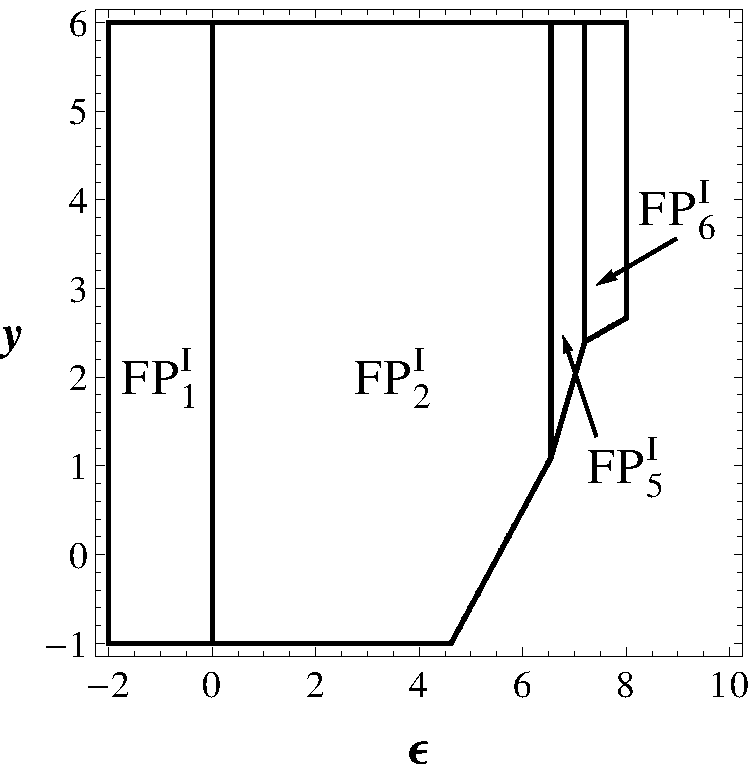
\includegraphics[width=6cm]{ThN.eps} 
  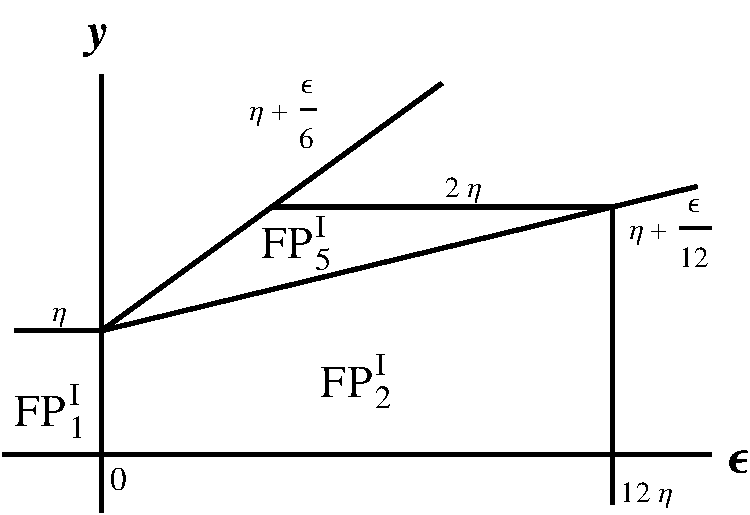
\includegraphics[width=7cm]{Stab_reg_RCHM.pdf} 
  \caption{Области устойчивости неподвижных точек в плоскости $(\eps,y)$ для модели быстро меняющегося поля скорости.}
  \label{fig:stab_rchm}
\end{figure}

Границы устойчивости для точки \fp{I}{6} могут быть вычислены только численно, поэтому мы их не включили.

The phase boundaries for the \fp{I}{6} can be obtained only in the numerical way and therefore they are not included. 

Точка \fp{I}{1} соответсвует свободной (Гауссовой) теории, в которой все взаимодейсвтия не приносят вклад и здесь пременима обычная теория возмущений.
Однако существование такой точки в РГ подходе является необходимым \cite{Vasiliev}.
В точке \fp{I}{2} коррелятор скорости не вносит вклад и эта точка соответсвует универсальному классу стандартного процесса протекания \cite{JanTau04}.
Остальные две неподвижные точки соответствуют новым нетривиальным режимам, для которых как флуктуации скорости, так и взаимодействие процесса протекания имеют значение.
На Рис. \ref{fig:stab_rchm} видно, что существование режима \fp{I}{5} в решающей степени зависит от ненулевого значения параметра $\eta$.


\fp{I}{1} corresponds to the free (Gaussian) theory for which all interactions are irrelevant 
and ordinary perturbation theory is applicable. However, existence of such point is necessary
condition for the RG approach \cite{Vasiliev}.
For the \fp{I}{2} the correlator of the velocity field is irrelevant and 
this point describes a standard DP universality class \cite{JanTau04}.
Remaining two fixed points represent nontrivial regimes, for which velocity
fluctuations as well as percolation interaction are relevant.
 In Fig. \ref{fig:stab_rchm} we observe that the realizability of the regime \fp{I}{5} 
crucially depends on the non-zero value of $\eta$.
%-------------------------------------------------------------------------------------------------------------------%
{\subsection{Тепловые флуктуации} \label{subsec:thermal}}
Для модели быстро меняющегося поля скорости рассмотрим специальный случай, соответствующий тепловым флуктуациям \cite{FNS}.
В этом случая характерен квадратичный закон дисперсии, для этого наложим на наш коррелятор скорости (\ref{eq:kernelD}) дополнительное условие 

Now we analyze a special case of the rapid-change model, which describes
thermal fluctuations \cite{FNS}. They
are characterized by quadratic dispersion law and in our choice of
velocity correlator (\ref{eq:kernelD}), an additional condition 
\begin{equation}
  \eta = 6 +y - \eps.
  \label{eq:cond_thermal}
\end{equation}
Области устойчивости неподвижных точек в плоскости $(\eps,y)$ изображены на рисунке \ref{fig:thermal}.
При физическом выборе параметров $d=3\mbox{ }(\eps=1)$ и $d=2\mbox{ }(\eps=2)$ возможен только режим, соответствующий чистому процессу перколяции.
Нетривиальные режимы \fp{I}{5} and \fp{I}{6} могут существовать лишь в нефизической области, для которой характерен выбор большого значения параметра $\eps$.
Численные результаты находятся в соответсвии с предыдущими работами \cite{AntKap08,AntKap10}.
Как было показано в \cite{HH00} тепловые флуктуации могут изменить картину устойчивости неподвижных точек, но для процесса протекания это не происходит.


has to be met. 
A phase structure in the plane $(\eps,y)$ is depicted in
Fig. \ref{fig:thermal}. For physical space dimensions 
$d=3\mbox{ }(\eps=1)$ and $d=2\mbox{ }(\eps=2)$ the only stable regime is that of pure DP.
The nontrivial regimes \fp{I}{5} and \fp{I}{6} are realized only in the nonphysical
region for large values of $\eps$. This numerical result confirms our
previous expectations \cite{AntKap08,AntKap10}. 
It was pointed out \cite{HH00} that
genuine thermal fluctuations can change IR stability of the given universality class. 
However, this is not realized for the percolation process itself.
\begin{figure}[h!]
  \centering
  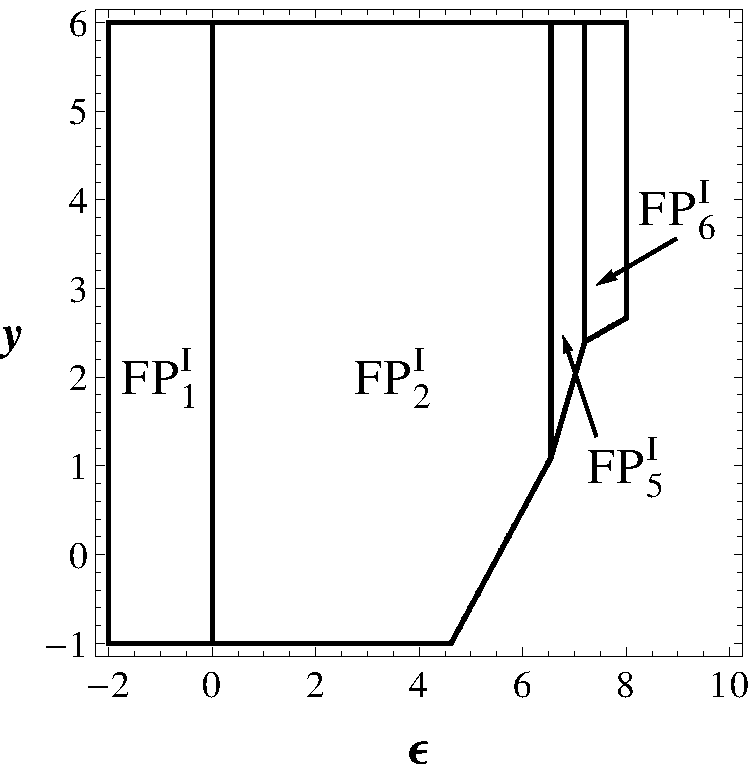
\includegraphics[width=6cm]{ThN.pdf}
  \caption{Области устойчивости неподвижных точек для процесса протекания с тепловыми флуктуациями в плоскости $(\eps,y)$. Обозначения неподвижных точек совпадают с случаем быстро меняющегося поля скорости в таблице \ref{tab:rchm}}
  \label{fig:thermal}
\end{figure}
%-------------------------------------------------------------------------------------------------------------------%
{\subsection{Замороженное поле скорости} \label{subsec:frm}}
Модель замороженного поля скорости получается из нашей общей модели выбором $u_1=1$.
В задаче переноса \cite{Ant00} этот случай соответсвует блужданиям в среде с дальним радиусом корреляции \cite{HonKar88}.
В данной модели мы имеем пять неподвижных точек, координаты которых представлены в таблице \ref{tab:frozen}.
Только три точки \fp{II}{1}, \fp{II}{2} и \fp{II}{4} оказываются ИК- притягивающими.

Frozen velocity limit is obtained for the choice $u_1=1$. 
In the formulation of an advection of density field
 \cite{Ant00}  it corresponds to the model of random walks in a random environment with long-range
 correlations \cite{HonKar88}.
In this case
five fixed points can found and their coordinates are listed in Table \ref{tab:frozen}. Only
the points \fp{II}{1}, \fp{II}{2} and \fp{II}{4} are IR stable.
\begin{table}[!ht ]
  \centering
  \setlength\extrarowheight{7pt}
  \begin{tabular}{| c||c|c|c|c |}
    \hline
    \fp{II}{} & $g_1$ & $g_2$ & $u_2$ & $a'$ \\
    \hline\hline
    \fp{II}{1} & $0$ & $0$ & NF& NF\\
    \hline
    \fp{II}{2} & $0$ & $\frac{2}{3}\eps$ & $0$ & $0$ \\
    \hline
    \fp{II}{3} & $\eps-y$ & $4 y $ & $1$ & $\frac{5 y - \eps }{\eps - y}$ \\
    \hline
    \fp{II}{4} & $4( 6 y - \eps )$ & $4 y$ & $\frac{4 \eps - 25 y + \sqrt{-8 \eps y + 49 y^2}}{8(\eps - 6y)}$ & $0$ \\
    \hline
    \fp{II}{5} & $4( 6 y - \eps )$ & $4 y$ & $\frac{4 \eps - 25 y - \sqrt{-8 \eps y + 49 y^2}}{8(\eps - 6y)}$  & $0$ \\
    \hline
    \end{tabular}
    \caption{Координаты неподвижных точек в модели с замороженным полем скорости.}
    \label{tab:frozen}
\end{table}
Точка \fp{II}{1} соответсвует свободной (Гауссовой) теории.
Ее область устойчивости

The fixed point \fp{II}{1} describes the free (Gaussian) theory. It is stable in the region
\begin{equation}
   y<0,\quad \eps < 0, \quad \eta < 0.
   \label{eq:free_frozen} 
\end{equation}
Для точки \fp{II}{2} поле скорости не вносит вклад, что соответсвует чистому процессу протекания.
Данная точка устойчива при 

For the \fp{II}{2}
the velocity field is irrelevant and the only 
relevant interaction is the nonlinearity of the percolation process. This FP is stable in
 the region
 \begin{equation}
   \eps > 6y, \quad \eps > 0,\quad \eps > 12\eta.
   \label{eq:DP_frozen}
\end{equation}

Точка \fp{II}{4} соответсвует нетривиальному режиму, для которого как поле скорости так и взаимодействие чистой модели дают вклад.
Области устойчивости точек \fp{II}{1} и \fp{II}{2} изображены на Рис. \ref{fig:frozen}.
Из-за того что для этих точек фактически можно перенбречь полем скорости, границы их областей устойчивости не зависят от значения параметра $\alpha$.
Область устойчивости точки \fp{ii}{4} может быть посчитанна только численна и она, конечно, зависит от $\alpha$.
На Рис. \ref{fig:frozen} видно, что корреляционный параметр $\eta$ в решающей степени влияет на границу между \fp{II}{2} и \fp{II}{4} областями.

 \fp{II}{4} embodies a nontrivial regime for which both velocity and
percolation interactions are relevant. The regions of stability for the \fp{II}{1} and \fp{II}{2} 
are depicted in Fig. \ref{fig:frozen}. Because for these two points
the velocity field could be effectively neglected, it directly follows that
 given boundaries could not depend on the value of parameter $\alpha$. The stability region
of \fp{ii}{4} can be computed only numerically and it turns out that it depends on $\alpha$. 
From Fig. \ref{fig:frozen} we observe that correlation parameter $\eta$ crucially affects
boundaries between \fp{II}{2} and \fp{II}{4}.
\begin{figure}[h!]
   \centering
   \begin{tabular}{ c c}
     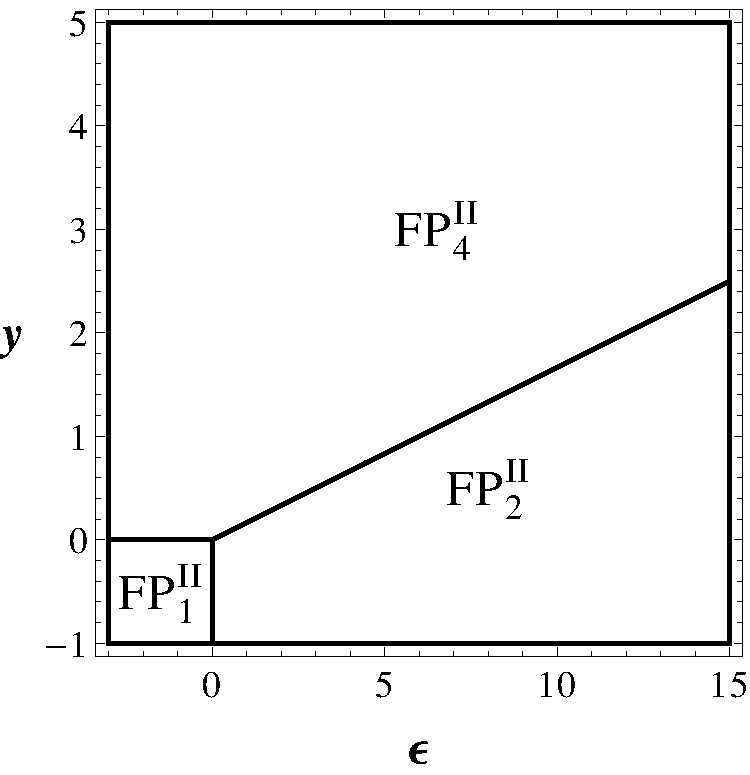
\includegraphics[width=6cm]{FVF_0.pdf}
     &
     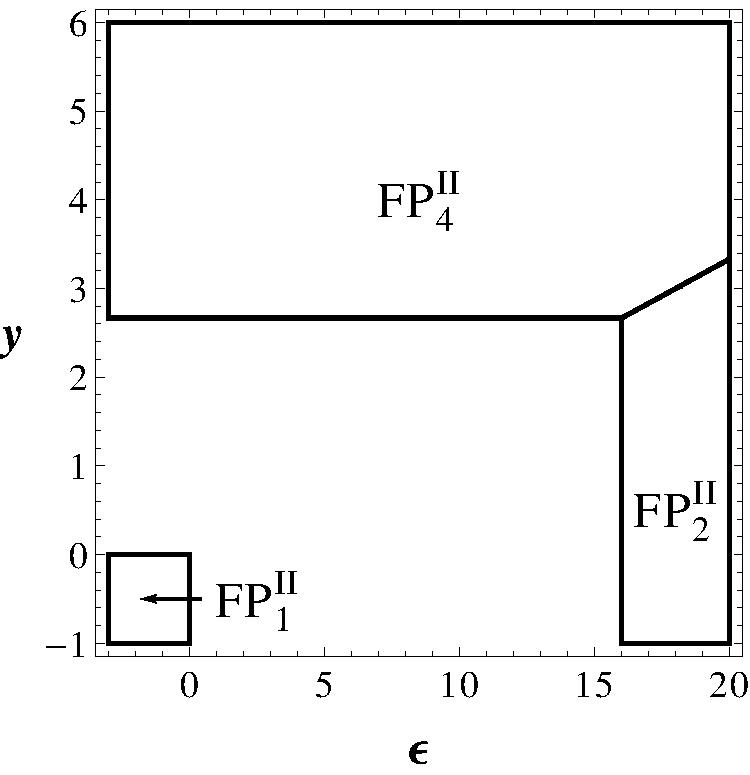
\includegraphics[width=6cm]{FVF_4-3.pdf}
   \end{tabular}
   \caption{Области устойчисости в плоскости $(\eps,y)$ для модели с замороженным полем скорости. Слева изображен случай $\eta=0$. Справа - $\eta=4/3$.}
   \label{fig:frozen}
\end{figure}
%-------------------------------------------------------------------------------------------%
{\section{} \label{sec:conclu}}
В данной работе мы изучали направленый процесс протекания в присутствии безвихревого поля скорости, коррелятор которого обладает длиннодействием.
Детально обсуждались способ построения и процедура мультипликативной ренормировки для данной модели. 

Было обнаружено, что в зависимости от значений размерности пространства $d=4-\eps$, показателей $y$ и $\eta$ наша модель демонстрирует различные типы критического поведения, связанные с различными классами универсальности.
Некаотрые из них уже хорошо известны: Гауссова (свободная) неподвижная точка, процесс протекания без перемешивания и процесс перемешивания пассивного скалярного поля.
Оставшиеся точки соответствуют новым классам универсальности, для которых актуальны как взоимодействие процесса протекания, так и перемешивание.

Было показано \cite{GV99} что аномальное критическое поведение разрушается когда значения параметров $\alpha$ и $y$ достаточно велики.
Следовательно допустимы только относительно маленькие значения ($\alpha \ll 1$) для нашей модели. 
Эта ситуация соответствует малым флуктуациям плотности $\rho$. Другими словами, предполагается, что скорость звука в жидкости значительно меньше скорости звука в системе (число Маха $\mathrm{Ma} \ll 1$).
Тем не менее мы считаем, что количественная картина при больших значениях сжимаемости останется прежней.
В качестве дальнейших исследований можно рассматривать задачу с дополнительными эффектами, такими как обратная связь на динамику перемешивающего поля, анизотропия или нарушение зеракльной симметрии.

Some of them are already well-known: the Gaussian (free) fixed point,
 a directed percolation without advection and a passive scalar advection. The remaining
 points correspond to new universality classes, for which an interplay
between advection and percolation is relevant.

It was shown \cite{GV99} that anomalous scaling behavior is destroyed when $\alpha$ and $y$ are large
enough. Therefore only relatively small values of
$\alpha$ are allowed ($\alpha \ll 1$) in our model. They correspond to small fluctuations of the density 
$\rho$, what is tacitly supposed in our investigation. In other words, it is assumed that the
 velocity of the fluid is much smaller than the velocity
of the sound in the system (the Mach number $\mathrm{Ma} \ll 1$). 
 Nevertheless we believe that a qualitative picture for
large values of compressibility should remain the same.
Further investigation should also take into account additional effects such as feedback on the dynamics of the
advecting field, anisotropies or broken mirror symmetry.

%-------------------------------------------------------------------------------------------%
%		Acknowledgment
%-------------------------------------------------------------------------------------------%
Данная работа была написа при поддержке гранта VEGA No. $1/0222/13$ Министерства образования, науки, исследований и спорта Республики Словакия, а также при поддержке исследовательского гранта No. 11.38.185.2014 Санкт-Петербургского государственного университета.

The work was supported by VEGA grant No. $1/0222/13$ 
 of the Ministry of Education, Science, Research and Sport of the Slovak Republic. N.~V.~A. and
  A.~S.~K. acknowledge Saint Petersburg State University for Research Grant No. 11.38.185.2014.
%--------------------------------------------------------------------------------------------------%
\begin{thebibliography}{99}
 \bibitem{Hin06} H.~Hinrichsen, Physica A {\bf 369}, 1 (2006).
 \bibitem{Stauffer} D.~Stauffer, A.~Aharony, {\it Introduction to Percolation Theory}
     (Taylor and Francis, London, 1992).
 \bibitem{HHL08} M.~Henkel, H.~Hinrichsen, S.~L{\"u}beck, 
     {\it Non-equilibrium phase transitions: Volume 1 – Absorbing phase transitions}, 
     (Springer, Dordrecht, 2008).
 \bibitem{Schlogl} F.~Schl\"ogl, Z. Phys. {\bf 253}, 147 (1972).
 \bibitem{Grassberger82} P.~Grassberger, Z. Phys. B: Condens. Matter {\bf 47}, 365 (1982).
 \bibitem{Gribov} V.~N.~Gribov, Sov. Phys. JETP {\bf 26}, 414 (1968).    
 \bibitem{Cardy} J. L. Cardy and R. L. Sugar, \emph{ J. Phys. A} {\bf 13}, L423–L427, (1980).
 \bibitem{Hinrichsen} H.~Hinrichsen, J. Stat. Mech.: Theor. Exp. P07066 (2007).
 \bibitem{Janssen81} H.~K.~Janssen, Z. Phys. B: Condens. Matter {\bf 42}, 151 (1981).
 \bibitem{Janssen96} H.~K.~Janssen, Phys. Rev. E {\bf 55}, 6253 (1997).
 \bibitem{RRR03} P.~Rupp, R.~Richter, I.~Rehberg, Phys. Rev. E {\bf 67}, 036209 (2003).
 \bibitem{TKCS07} K.~A.~Takeuchi, M.~Kuroda, H.~Chat, M.~Sano, Phys. Rev. Lett. {\bf 99}, 234503 (2007).
 \bibitem{FGV01} G.~Falkovich, K.~Gaw\c{e}dzki, M.~Vergassola, Rev. Mod. Phys. {\bf 73}, 913 (2001). 
 \bibitem{Landau_fluid} L.~D.~Landau and E.~M.~Lifshitz, {\it Fluid Mechanics} (Pergamon Press, 1959).
 \bibitem{Frisch} U.~Frisch, {\it Turbulence: The Legacy of A. N. Kolmogorov} (Cambridge University Press, Cambridge, 1995). 
 \bibitem{Monin} A.~S.~Monin and A.~M.~Yaglom, {\it Statistical Fluid Mechanics:Vol 2}
    (MIT Press, Cambridge, 1975). 
 \bibitem{Ant99} N.~V.~Antonov, Phys. Rev. E {\bf 60}, 6691 (1999).
 \bibitem{Benzi09} R.~Benzi and D.~R.Nelson", Physica D {\bf 238}, 2003 (2009).
 \bibitem{Pig12} S.~Pigolotti and R.~Benzi and M.~H.~Jensen and D.~R.~Nelson, 
    Phys. Rev. Lett. {\bf 108}, 128102 (2012).
 \bibitem{Volk14} R.~Volk and C.~Mauger and M.~Bourgoin and C.~Cottin-Bizonne
	      and C.~Ybert and F.~Raynal, Phys. Rev. E {\bf 90}, 013027 (2014).
 \bibitem{depietro15} M.~De~Pietro and M.~A.~T.~van~Hinsberg and L.~Biferale and
	      H.~J.~H.~Clercx and P.~Perlekar and F.~Toschi, Phys. Rev. E {\bf 91}, 053002 (2015).
 \bibitem{Ant00} N.~V.~Antonov, Physica D {\bf 144}, 370 (2000).
 \bibitem{AntKap08} N.~V.~Antonov, V.~I.~Iglovikov, A.~S.~Kapustin, J. Phys. A: Math. Theor. {\bf 42}, 135001 (2008).
 \bibitem{AntKap10} N.~V.~Antonov, A.~S.~Kapustin, J. Phys. A: Math. Theor. {\bf 43}, 405001 (2010).
 \bibitem{Ant11} N.~V.~Antonov, A.~S.~Kapustin, A.~V.~Malyshev, Theor. Math. Phys. {\bf 169}, 1470 (2011).
 \bibitem{DP13} M.~Dan\v{c}o, M.~Hnati\v{c}, T.~Lu\v{c}ivjansk\'{y} and L.~Mi\v{z}i\v{s}in, Theor. Math. Phys. {\bf 176}, 898 (2013).
 \bibitem{Vasiliev} A.~N.~Vasil'ev, {\it The Field Theoretic Renormalization Group in Critical Behavior Theory and Stochastic Dynamics}
 \bibitem{JanTau04} H.~K.~Janssen, U.~C.~T{\"a}uber, Ann. Phys. {\bf 315}, 147 (2004).
 \bibitem{Doi} M.~Doi, J. Phys. A {\bf 9}, 1465 (1976); {\it ibid.} {\bf 9}, 1479 (1976).        
 \bibitem{Janssen76} H.~K.~Janssen, Z. Phys. B: Condens. Matter {\bf 23}, 377 (1976).
 \bibitem{deDom76} C.~De~Dominicis, J. Phys. Colloq. France {\bf 37}, C1-247 (1976).
 \bibitem{Janssen79} H.~K.~Janssen, {\it Dynamical Critical Phenomena and Related Topics},
    Lect. Notes Phys. {\bf 104}, (Springer, Heidelberg, 1979).
 \bibitem{Zinn} J.~Zinn-Justin, \textit{Quantum Field Theory and Critical Phenomena} (Oxford University Press, Oxford, 1989).   
 \bibitem{AdzAnt98} L.~Ts.~Adzhemyan, N.~V.~Antonov, Phys. Rev. E {\bf 58}, 7381 (1998).   
 \bibitem{Amit} D. J. Amit and V. Mart\'in-Mayor, {\it Field Theory, the Renormalization Group and Critical Phenomena}
 (World Scientific, Singapore, 2005). 
 \bibitem{Tauber2014} U.~T{\"a}uber, {\it Critical Dynamics: A Field Theory Approach to Equilibrium
 	      and Non-Equilibrium Scaling Behavior}
 	      (Cambridge University Press , New York, 2014).
 \bibitem{AAK94} L.~Ts. Adzhemyan, N.~V.~Antonov, T.~L.~Kim, Theor. Math. Phys. {\bf 100}, 1086 (1994).
 \bibitem{ABG96} N.~V.~Antonov, S.~V.~Borisenok, V.~I.~Girina, Theor. Math. Phys. {\bf 106}, 75 (1996).
 \bibitem{AV97} N.~V.~Antonov, A.~N.~Vasil'ev, Theor. Math. Phys. {\bf 110}, 97 (1997).
 \bibitem{FNS} D.~Forster, D.~R.~Nelson, M.~J.~Stephen, Phys. Rev. A {\bf 16}, 732 (1977).
 \bibitem{HH00} M.~Hnatich, J.~Honkonen, Phys. Rev. E {\bf 61}, 3904 (2000).
 \bibitem{HonKar88} J.~Honkonen and E.~Karjalainen, J. Phys. A: Math. Gen. {\bf 21}, 4217 (1988). 
 \bibitem{GV99} K.~Gaw{\c{e}}dzki, M.~Vergasssola, Physica D {\bf 138}, 63 (1999).
\end{thebibliography}

\end{document}